\documentclass[portrait]{seminar}
\newtheorem{thm}{Theorem}[section]
\newtheorem{lem}[thm]{Lemma}
\newtheorem{cor}[thm]{Corollary}
\newtheorem{prop}[thm]{Proposition}
\newtheorem{claim}{Claim}
\newtheorem{ex}{Example}
\newtheorem{defn}[thm]{Definition}
\usepackage{epic,eepic,colordvi,psfig}
\def\theenumii{\arabic{enumi}.\arabic{enumii}}
\def\labelenumii{\arabic{enumi}.\arabic{enumii}}
\background{White}
\textBlack
\portraitonly
\slideframe{none}
%\setlength{\textwidth}{270mm} 
\setlength{\textheight}{200mm} 
%\paperheight 19cm
\paperwidth 27cm
\renewcommand\slideleftmargin{-7.1cm}
\def\thepage{\arabic{page}}
\begin{document}

\title{Using Approximation Hardness to Achieve Dependable 
Computation\thanks{Supported by DARPA  F30602-97-1-0205}}
%\author{ }
\date{ }

%\begin{slide*}{}
\maketitle

\begin{center}
\Green{
$$\begin{array}{cc}
\mbox{Mike Burmester} & \mbox{Yvo Desmedt, Yongge Wang}\\
\mbox{Dept. of Maths} & \mbox{Dept. of EE \& CS}\\
\mbox{Univ. of London} & \mbox{Univ. of Wisconsin}\\
& \mbox{Milwaukee}
\end{array}$$}

\vskip 0.5cm

October 8, 1998
\end{center}




\newpage

\section*{\Green{Overview}}

\Red{
\begin{enumerate}
\item Motivation
}
\Blue{
\begin{enumerate}
\item Network reliability and security
\item Secure distributed computation needs a different model
\item Problem is {\bf NP}-hard
\item A possible application
\end{enumerate}
}\Red{
\item Some details
}
\Blue{
\begin{enumerate}
\item Main concept
\item Main idea
\item Constructing AND/OR graphs
\end{enumerate}
}\Red{
\item Open problems
\end{enumerate}
}
\newpage

\Red{\section{Motivation}}

\Blue{\subsection{Network reliability and security}}

\begin{itemize}
\vskip -10pt
\item against passive adversaries (destructing nodes and edges): 
needs $k+1$-connectivity

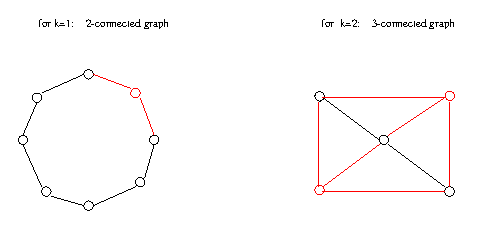
\psfig{file=slidepic1.eps}

\vskip -10pt
\item against Byzantine (lying) nodes: needs $2k+1$-connectivity

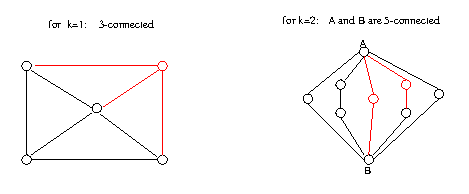
\psfig{file=slidepic2.eps}
\end{itemize}

\nopagebreak
E.g., used in ``mental games''.

\newpage
\Blue{\subsection{Secure distributed computation needs a different model}}

The airplane's next position 
$s=s_0+v\times t+\frac{1}{2}a\times t^2$
\begin{itemize}
\vskip 3pt
\item $s_0$: current position
\vskip 3pt
\item $v$: speed
\vskip 3pt
\item $a$: acceleration, here $a=0$
\end{itemize}

\vskip 0pt
$$\begin{array}{ll}
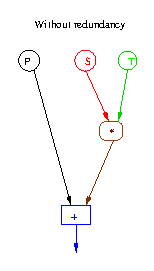
\psfig{file=slidepic4.eps} &
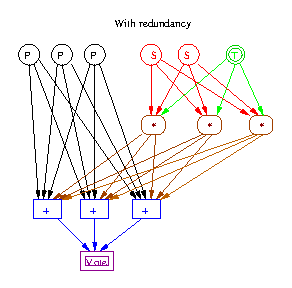
\psfig{file=slidepic5.eps}
\end{array}$$

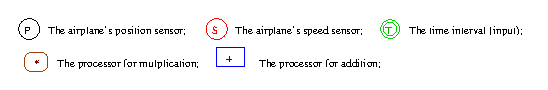
\psfig{file=slidepic6.eps}

\newpage
Wang-Desmedt-Burmester use an AI concept:

\vskip 5pt
\begin{center}
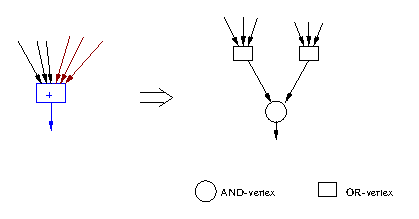
\psfig{file=slidepic7.eps}
\end{center}

\vskip -20pt
\noindent
a vertex is: a sensor, or a process, or a dedicated computer


\begin{defn}
\Red{An {\rm AND/OR graph} \\
$G_{\wedge\vee}(V_\wedge, V_\vee, INPUT, output; E)$ is a
directed graph with:
\begin{itemize}
\item  a set $V_\wedge$ of {\rm $\wedge$-vertices}
\item a set $V_\vee$ of {\rm $\vee$-vertices}
\item a set $INPUT$ of {\rm input vertices}, $indegree=0$
\item an {\rm output vertex} $output\in V_\vee$, $outdegree=0$
\item  and a set of {\rm directed edges} $E$
\end{itemize}
}
\end{defn}

\Blue{\subsection{Problem is {\bf NP}-hard}}
\begin{itemize}
\item Deciding whether a given graph is $k$-connected, i.e.,
has $k$ disjoint paths from each node to each node, is in {\bf P}
\item The equivalent problem for AND/OR graph is {\bf NP}-complete
(Wang-Desmedt-Burmester)
\item Implication:

Given an AND/OR graph, finding whether there are $k$ disjoint solution
graphs is {\bf NP}-hard.
\end{itemize}

\newpage
\begin{defn}
\Red{Let $G_{\wedge\vee}(V_\wedge, V_\vee, INPUT, output; E)$ be
an AND/OR graph.
A \Red{solution graph} $P=(V_P, E_P)$ is a minimum subgraph 
of $G_{\wedge\vee}$ satisfying the following conditions:
\begin{enumerate}
\item $output\in V_P$.
\item For each $\wedge$-vertex $v\in V_P$,  all incoming
edges of $v$ in $E$ belong to $E_P$.
\item For each $\vee$-vertex $v\in V_P$,  there is 
exactly one incoming edge of $v$ in $E_P$.
\item There is a sequence
of vertices $v_1, \ldots, v_n\in V_P$ such that
$v_1\in INPUT, v_n=output$, and 
$(v_i\!\rightarrow\!v_{i+1})\in E_P$
for each $i<n$.
\end{enumerate}
Moreover, two solution graphs $P_1$ and $P_2$ are
{\rm vertex disjoint} if $(V_{P_1}\cap V_{P_2})
\subseteq (INPUT\cup \{output\})$.}

\newpage
\Red{An AND/OR graph is called {\rm $k$-connected} if
the following conditions are satisfied.
\begin{enumerate}
\item There are $k$ vertex disjoint solution graphs in $G_{\wedge\vee}$.
\item There do not exist $k+1$ vertex disjoint solution 
graphs in $G_{\wedge\vee}$.
\end{enumerate}
}
\end{defn}

\newpage
\Blue{\subsection{A possible application}}
\begin{itemize}
\item If an AND/OR graph has $k+1$ ($2k+1$) disjoint solution
graphs, then as for the network case, it can guarantee
reliability.
\item Now if the AND/OR graph does not have $k+1$ ($2k+1$) disjoint solution
graphs, then a polynomial time enemy may still fail.

Indeed it may be hard to find $k$ \Red{DISJOINT} solution graphs.

\item \Red{GOAL}: make a graph that has ONLY $k^\prime<k$ disjoint
solution graphs, but is secure against an adversary
who can corrupt $k$ nodes.

\item \Red{OBTAINED RESULTS}: 
\begin{enumerate}
\item yes if $k=ck^\prime$, $c>1$ is any constant
\item yes if $k=(k^\prime)^{1+\varepsilon}$, $1>\varepsilon>0$
is certain constant
\end{enumerate}
\end{itemize}

\newpage
\Red{\section{Some details}}

\Blue{\subsection{Main concept}}

\Red{Vertex Separator}$\{v_{i_1}, v_{i_2},\ldots, v_{i_k}\}$  
of AND/OR graphs if

\vskip 10pt
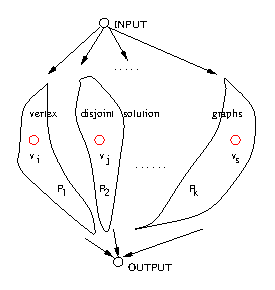
\psfig{file=slidepic8.eps}

\vskip 10pt
\noindent
where $\{P_1, P_2, \ldots, P_k\}$ is a maximum set of vertex
disjoint solution graphs, i.e.,  $\exists \pi: \forall i
(1\le i\le k): v_{\pi(i)}\in V_{P_i}$

\newpage
\Blue{\subsection{Main idea}}

\vskip 10pt

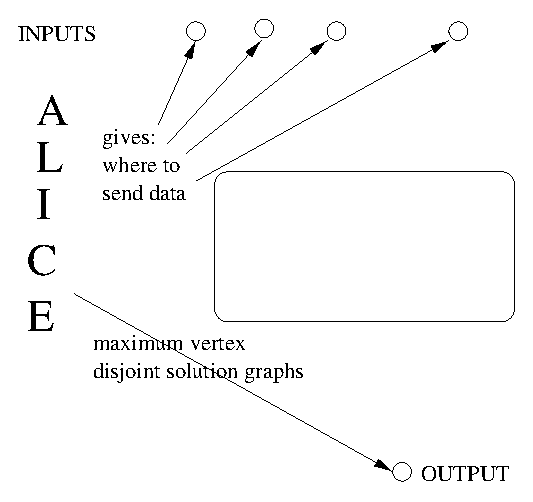
\psfig{file=slidepic9.eps}

\vskip -5.2cm
{\small
\hskip 3.5cm Graph such that:

\hskip 3cm $-)$ is $k^\prime$ connected

\hskip 3cm \mbox{$-)$ hard to find $k$ vertex set $U$:}

\hskip 3cm \ \ \ $\exists V_{sep}:\ |U\cap  V_{sep}|>| V_{sep}|/2$

\hskip 3cm $-)$ it achieves the desired 

\hskip 3cm  \ \ \ computation
}

\vskip 3cm
We consider $k=ck^\prime$, $c$ a constant

\newpage
\Blue{\subsection{Constructing AND/OR graphs}}

\Red{\begin{thm}
Given an AND/OR graph  \\
$G_{\wedge\vee}(V_\wedge, V_\vee, INPUT, output; E)$,
it is {\bf NP}-hard to compute a vertex set 
$S^\prime\subseteq (V_\wedge\cup V_\vee)$:
\begin{enumerate}
\item If $G_{\wedge\vee}$ is $k^\prime$-connected then 
$|S^\prime|\le ck^\prime$.
\item $\exists$ vertex separator $S$ of $G_{\wedge\vee}$, 
$|S\cap S^\prime|\ge \frac{k^\prime}{2}.$
\end{enumerate}
\end{thm}
}

\noindent
PROOF: USE: Approximating IS is hard 

\noindent
Given graph $G^\prime(V^\prime, E^\prime)$: $V^\prime=\{v_1, \ldots, v_n\}$,
we construct an AND/OR graph $G^{\prime\prime}_{\wedge\vee}$:

\vskip 10pt
\Red{(*) A set of vertex disjoint solution graphs in 
$G^{\prime\prime}_{\wedge\vee}$ implies a set of independent
vertices in $G^\prime$}, as follows

\vskip 20pt

\begin{itemize}
\item $INPUT^{\prime\prime}=\{I_i,I_{i,j}: i,j=1, \ldots n\}$
\item $V_\vee^{\prime\prime}=\{output\}$
\item $V_\wedge^{\prime\prime}= 
\{u_{i,j}:  i,j=1, \ldots n\} \cup 
\{u_i: i=1, \ldots,n\}$
\end{itemize}

\newpage

%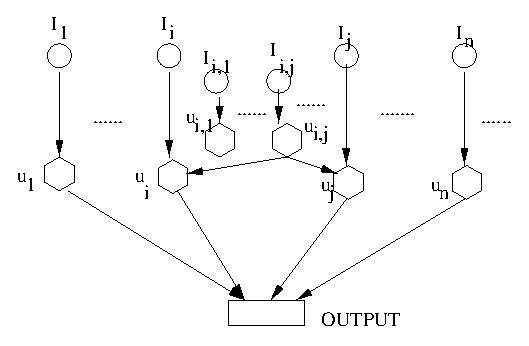
\psfig{file=slidepic10.eps}

\input{slidepic10.eepic}

\vskip -30pt\ 
\begin{itemize}
\item  and $E^{\prime\prime}$ be the set of 
\begin{enumerate}
\item For each $i=1,\ldots, n$, an edge
$I_i\!\rightarrow\! u_i$.
\item For each  pair $i,j=1,\ldots, n$, 
an edge $I_{i,j}\!\rightarrow\! u_{i,j}$.
\item For each pair $i,j=1,\ldots, n$, 
such that $(v_i,v_j)\in E^\prime$,
four edges $u_{i,j}\!\rightarrow\! u_i$,
$u_{i,j}\!\rightarrow\! u_j$,  $u_{j,i}\!\rightarrow\! u_i$,
and $u_{j,i}\!\rightarrow\! u_j$.
\item For each $i$, an edge 
$u_i\!\rightarrow\! output^{\prime\prime}$.
\end{enumerate}
\end{itemize}


\newpage

\Blue{\subsection*{Some results on approximation hardness}}

Given a graph $G(V,E)$, assume that the size of the maximal
independent set of $G$ is $k^\prime$, then:
\begin{itemize}
\item it is {\bf NP}-hard to find a maximal independent 
set of $G$
\item it is {\bf NP}-hard to find an independent set $V^\prime\subset V$
with $|V^\prime|\le \frac{k^\prime}{c}$, $c>1$ is a constant 
\end{itemize}

We show the following

\Red{
\begin{itemize}
\item it is {\bf NP}-hard to find a set $V^\prime\subset V$
such that 
\begin{enumerate}
\item $|V^\prime|\le ck^\prime$, $c>1$ is a constant
\item $V^\prime$ contains an independent set
of size $\frac{k^\prime}{2}$ 
\end{enumerate}
\end{itemize}
}

\makebox[5mm]{}

\newpage
\Red{\section{Open problems}}

\begin{itemize}
\item Practical solution
\item Constructing AND/OR graphs against dynamic adversaries
\end{itemize}

%\end{slide*}
\end{document}


